%As  !TEX root = ../../report.tex
\section{Generating implicit ratings}
\label{sec:implementation-implicit}

In this section we continue solving the problem of generating ratings based on
implicit feedback found in analytics logs, as defined in
Section~\ref{implicit-feedback}. Our goals are two-fold:

\begin{itemize}
  \item Find novel ways of creating implicit ratings, remedying as many
  weaknesses and challenges, depicted in Section~\ref{implicit-weaknesses}, as
  possible
  \item Customize existing and new algorithms to our fashion domain, described
  in Section~\ref{motivation}
\end{itemize}

The most important factor when creating ratings is to understand which implicit
data are available and their implications on user preferences. In order to best
understand the data one should do a quantitative study as presented in
Chapter~\ref{sobazaar-data}, but always keeping in mind the domain in question.
When an understanding is obtained one can begin selecting features capturing
the wanted properties and use these generalizations in order to generate
ratings for different users inhabiting unique patterns and product
interactions.

Then, upon evaluation of conversion features we can do an initial analysis
without any metrics by attempting to answer the question \textit{does this
generalization capture the domain and data properties?}
One such generalization, often done, is counting the number of a specified
activity on an item, correlating it with preference. In the case of SoBazaar
we've seen that a higher number of clicks yields a higher probability of
purchasing an item, thus we can use the number of clicks as a feature in
generating ratings - correlating a higher number of clicks to a higher rating.

Other properties, which we will discuss in this section and consequently
utilize, found in the \textit{fashion store aggregation} domain are:

\begin{itemize}
  \item Items have a short lifespan, due to:
  \begin{itemize}
    \item Seasons
    \item Fashion and trends
    \item Sales and price fluctuations
  \end{itemize}
  \item Items are not bought regularily, as with food and other convenience
  products
  \item Users are cost and brand-aware
\end{itemize}

Given a good set of chosen features we should, for all users that have
interacted with various items, obtain a well-distributed list of ratings - and
with more implicit feedback available for a user, we should obtain a higher
probability of the user having an unique set of ratings. This is easily seen in
the scenario where we do not consider social-graphs between users, and we have
two users $u_1$ and $u_2$ who has the equal implicit feedback - e.g. they
viewed the same items. If we only use global features, such as item popularity,
we have no way of giving unique ratings to the two users. However, if we
instead look at user-features such as \textit{when} did the users last look at
the items and \textit{in which order}, we have a higher probability of
obtaining unique sets of ratings.

When ratings are not explicit, the implicit ratings becomes the recommender
systems equivalent of a ground truth and all later stages in the recommender
pipeline (See Section~\ref{}) are dependent on the ratings representing a users
preferences. This highlights the importance of generating high quality ratings
and selecting good features and methods for doing so.

\subsection{Improving mapping of event types}

In Section~\ref{implicit-binary-domains} Pranab Ghosh proposes a global rating
mapping without any specific justification of why the different values are
chosen~\cite{pkghost2014implicit}. In order to use this method we wanted our
weighting of various events to be grounded in statistical properties found in
the dataset. Further we would like to create ratings on a continuous scale
between a min and max-value for the given event, not manually define levels of
scores. This way we could use a \textit{penalization function}, that based on
our selected feature ensured an even distribution between the minimum and
maximum value for the event in question. For example giving an often clicked
product for a user the maximum value and conversely the minimum value for
infrequent clicks.

To select good weights we thus considered the probability of each event that we
wanted to base our ratings on. These events were the ones having a
\textit{product id} as well as possibly inhabiting the implicit properties
described above. Instead of manually map events to an arbitrary score we used
the probability obtaining the given event type, given all events. Thus, our
score mapping looks like:

\begin{table}[H]
  \centering
  \begin{tabular}{llll}
    \toprule
      Event type & Probability & Min & Max \\
    \midrule
      \textit{product\_detail\_clicked}     & $\frac{25416}{40686} \approx 62$  & 0   & 62  \\[1.5ex]
      \textit{product\_wanted}              & $\frac{13252}{40686} \approx 33$  & 62  & 95  \\[1.5ex]
      \textit{prodcut\_purchase\_intended}  & $\frac{2018}{40686} \approx 5$    & 95  & 100 \\
    \bottomrule
  \end{tabular}
\end{table}

Notice that the total number of events having a product id is 40686, and the
sum of all three fractions is 1, thus covering 100\% of all events.

\subsection{Penalizing features}

How then do we distribute the feature-values  between the min and max limits
above? In our first implementation we use a \textit{linear penalization}
function, set in such a way that $0 \leq p(x) \leq 1$ and $0 \leq x \leq M_u$
where $M_u$ is the maximal observed value for user $u$ of the feature in
question, defined as:

\begin{equation}
  p(x, u) = \frac{x}{M_u}
\end{equation}

By considering penalization we also implicitly add negative feedback to events.
This is an important aspect to keep in mind when working with implicit
feedback, as discussed in Section~\ref{implicit-feedback} as modern recommender
engines work better when we are assuming ratings are based on both positive and
negative feedback.

Given $p(x, u)$ we formalize an equation for finding $S_e(x, u)$, the score
given to event $e$ after penalization, given a max $M_u$ and min $m_u$ value.

\begin{equation}
  S_e(x,u) = M_e - (M_e - m_e) \cdot p(x, u)
\end{equation}

The last component needed is normalizing the ratings. Which is described in
Equation~\ref{eq-normalization}. And now we have all components ready in order
to do a rating generation.

\subsection{Considering recentness}

In order to see all parts working together, we imagine an example where a user
has six events on three items, as presented in the table below. The ratings are
normalized between 1 and 5 and the product IDs are there for illustrative
purposes. We choose to look at the number of days since the user did the event
in question as the implicit feature, where $x=0$ means the event was registered
today (or as the most recent) and in our example $x=14$ is the oldest event
happening two weeks ago.

\begin{table}[H]
  \centering
  \begin{tabular}{llllll}
  \toprule
  Event type & Product ID & x (days) & P(x) & Score & Rating \\
  \midrule
  \textit{product\_purchase\_intended}  & 1 & 0   & $\frac{0}{14} = 0.00$  & 100 & 5.00 \\[1.5ex]
  \textit{product\_purchase\_intended}  & 2 & 3   & $\frac{3}{14} = 0.21$  & 98.95 & 4.96 \\[1.5ex]
  \textit{product\_wanted}              & 2 & 7   & $\frac{7}{14} = 0.50$  & 78.5 & 4.14 \\[1.5ex]
  \textit{product\_detail\_clicked}     & 1 & 0   & $\frac{0}{14} = 0.00$  & 62 & 3.48 \\[1.5ex]
  \textit{product\_detail\_clicked}     & 3 & 7   & $\frac{7}{14} = 0.50$  & 31 & 2.24 \\[1.5ex]
  \textit{product\_detail\_clicked}     & 2 & 14  & $\frac{14}{14} = 1.00$ & 62 & 1.0  \\
  \bottomrule
  \end{tabular}
  \caption{Showing penalizations and ratings on example data}
  \label{implicit-ratings-example}
\end{table}

When finally selecting a rating for the user/product pair, we choose the
one yielding the highest value for the given product. Hence for the three items
with IDs 1, 2 and 3 above we obtain the ratings 5.00, 4.96 and 2.24, respectively.

Using the same method on the SoBazaar dataset yields the following distribution
of ratings, where we group ratings together into 150 different bins - thus
every bin having an interval size of 0.0267:

\begin{figure}[H]
  \centering
  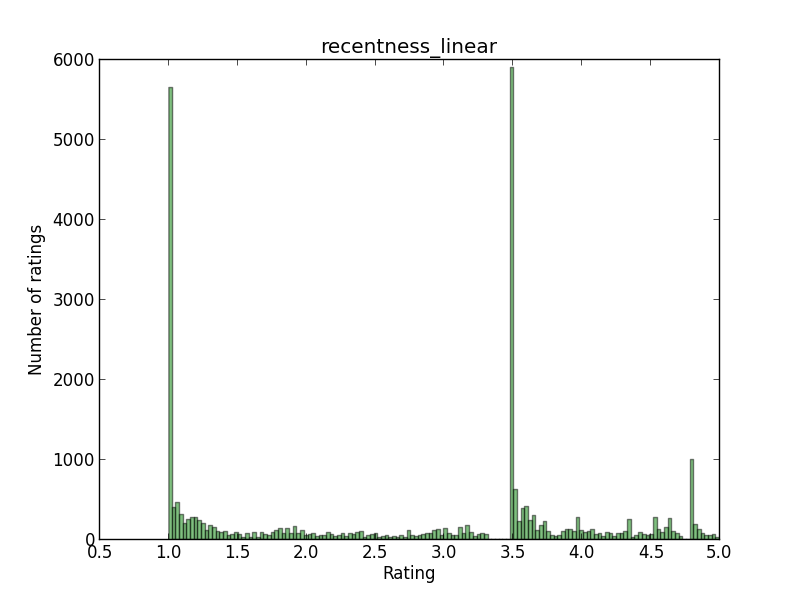
\includegraphics[scale=0.6]{image/dist-recentness-linear}
  \caption{Distribution of ratings using number of days since event as feature
  and a linear penalization function}
\end{figure}

We can see two ratings are widely more popular than others: 3.48 and 1.0. This
makes sense, as every user that has more than two clicks registered are
guaranteed to have the penalizations 1.0 and 0.0 apparent. As this is an
obvious weakness we change our penalizations such that $M_u$ and $m_u$ are not
longer based on the oldest and most recent events for user $u$, but rather the
oldest and newest event in the dataset globally. Changing these factors yield
the following distribution:

\begin{figure}[H]
  \centering
  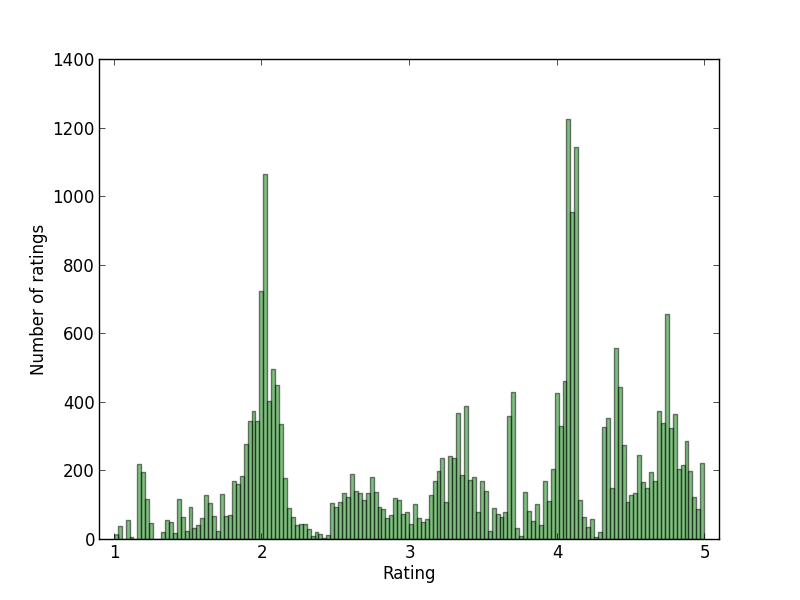
\includegraphics[scale=0.6]{image/dist-recentness-linear-global}
 \caption{Distribution of ratings using number of days since event, a linear
 penalization function and global min/max feature-values}
  \label{fig:dist-recentness-linear-global}
\end{figure}

This is a much more interesting result, having an more even distribution of
ratings with few gaps. The average rating is \textit{3.29} with a median
\textit{3.37}. The weakness in these results however is easy to spot given the
scenario when a user is absent from the application over a longer time and then
returns. In this scenario all the items the user has previously looked at,
wanted or bought will all suffer from large penalization values - and hence low
ratings, since the x for all items is very high. In addition the method does
not scale well, unless one limit the $M_u$ value, so that the difference
between two adjacent x values are significant. As SoBazaar is a relatively new
application this proved not to be a problem with our experiments, but given a
larger dataset with older events we would recommend testing $M_u = \min(O_e,
L)$ where $O_e$ is the number of days since the oldest event and $L$ is the
limit, set at e.g. 200.

In order to mitigate the returning user problem we adjust our feature to
instead consider the ordering of events for user $u$. This way, given $n$
events registered for this user, the newest event would obtain $x=0$ and the
oldest $x=n$. We continue to use a linear penalization function, which yields
the following distribution:

\begin{figure}[H]
  \centering
  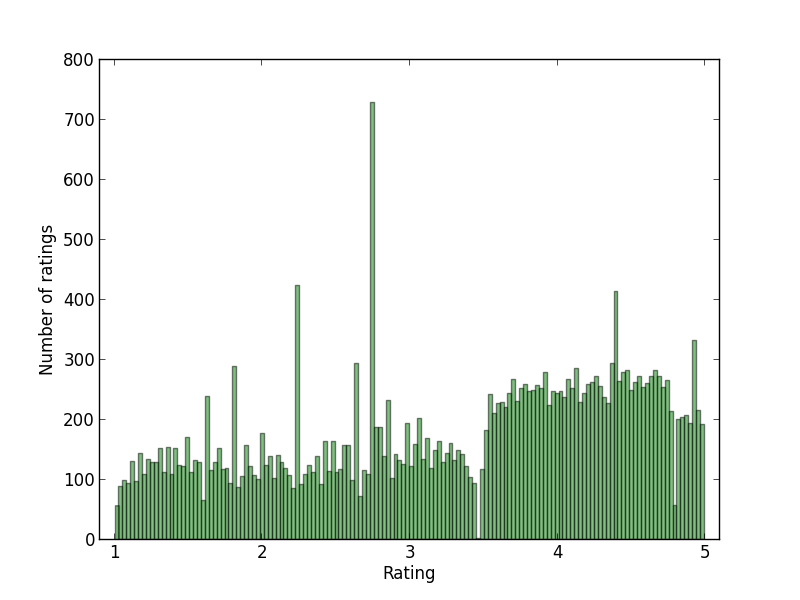
\includegraphics[scale=0.6]{image/dist-count-linear}
  \caption{Distribution of ratings using ordering of events, and a linear
 penalization function}
  \label{fig:dist-count-linear}
\end{figure}

With much the same average and median values at \textit{3.26} and \textit{3.45}
respectivly, we still have a distribution with a unique pattern where the
ratings are more evenly distributed (the largest bin contains 700 ratings in
the given interval, compared to Figure ~\ref{dist-recentness-linear-global}
where the same number is 1250.)

\subsubsection{Penalization with logistic functions}

So far we've seen ratings generated by looking at the event recentness,
capturing important factors such as items having a short life-time and users
frequently shopping for different occasions and hence different types of
clothes. However, we want to improve the penalization function in order to
capture the following properties in our domain:

\begin{itemize}
  \item Recent events should count more towards a good rating, compared to old
  events.
  \item Seasons change at a fixed interval, and clothes goes out of season in
  the matter of weeks.
  \item A user may look at multiple clothes at once, comparing them and finding
  them all quite interesting.
\end{itemize}

When using a linear function the difference in penalization between the two
most recent items are equal to the difference between the oldest two items.
However, intuitively we consider a user to have multiple relevant items
concurrently and we know that in domains such as technology, fashion and other
consumer-products an item has an age of relevancy, somewhat metaphoric to a
seasonal threshold. An example of this could be a fashion store recommending
warm clothes in the months between December to March, but then want to "change"
product pool based on the users behaviours --- who are probably looking for
lighter clothes (changing season).

In order to mimic this behaviour we introduce a logistic function, which is a
mathematical function having an "S" shape and a common special case of the more
general sigmoid-function. In its most simplest case the logistic function is
defined as:

% Vertical alignment of equation and plot.
\begin{figure}[H]
  \centering
  \noindent\begin{minipage}{.45\textwidth}
    \begin{tikzpicture}
      \begin{axis}
      \addplot[black,xlabel=$x$,ylabel=$f(x)$] {1/(1+exp(-x))};
      \end{axis}
    \end{tikzpicture}
  \end{minipage}
  \begin{minipage}{.45\textwidth}
  \begin{align}
    \label{logistic-function}
    f(x) = \frac{1}{1+\exp^{-x}}
  \end{align}
  \end{minipage}
  \caption{Logistic function having a S-shape with y-values ranging
  from 0 to 1.}
\end{figure}

Here the value of $f(x)$ is asymptotically limited between 0 and 1, dependent
on the value of $x$. The steepest point of the curve happens when $x=0$. By
adjusting the exponent of $e^{(-x)}$ we can skew the curve in order to map to our
data, giving us a \textit{function of relevancy} ranging from an item being
very relevant ($f(x)=0$) and not relevant ($f(x)=1$).

By adding two variables to the logistic function we can fine tune both the
steepness and range of $f(x)$. Hence we adjust Equation~\ref{logistic-function}
to include $s$, the \textit{steepness coefficient}, and $c$, the \textit{shift
coefficient}.

\begin{equation}
  p(x) = \frac{1}{1+\exp^{-s(x - c)}}
\end{equation}

In the standard sigmoid function these are $1$ and $0$ respectively, but by
adjusting $s$ closer to 0 we decrease the steepness, creating a more gradual
curve. Setting the $c$ to a larger number we shift the steepest point of the
curve to $x=c$, hence if we set $c$ to $20$, the steepest point (largest
acceleration) in our curve would be located when $x=20$.

We can manually try to set the steepnes and shift coeffiecients based on the
behaviour seen in the dataset provided. Using the data provided in
Table~\ref{implicit-ratings-example} we can again try to calculate the ratings
and penalizations. We set the steepness coefficient to be $0.8$, thus having a
curve that is not too steep yielding a good distribution. This constant works
well when the shift coefficient is low ($c \lessapprox 10$), however if the
shift coefficient increases the steepness should decrease. In our dataset we
found finding a fixed ratio between the steepness and shift worked best. The
shift is set at $M/2$, where $M$ equals the number of days between the oldest
and most recent event, in our example equalling 7.

\begin{table}[H]
  \centering
  \begin{tabular}{llllll}
  \toprule
  Event type & Product ID & x (days) & P(x) & Score & Rating \\
  \midrule
  \textit{product\_purchase\_intended}  & 1 & 0   & $\frac{1}{1 + \exp^{-0.8(0*7)}} = 0.00$  & 100 & 5.00 \\[1.5ex]
  \textit{product\_purchase\_intended}  & 2 & 3   & $\frac{1}{1 + \exp^{-0.8(3*7)}} = 0.03$  & 99.85 & 4.99 \\[1.5ex]
  \textit{product\_wanted}              & 2 & 7   & $\frac{1}{1 + \exp^{-0.8(7*7)}} = 0.50$  & 78.5 & 4.14 \\[1.5ex]
  \textit{product\_detail\_clicked}     & 1 & 0   & $\frac{1}{1 + \exp^{-0.8(0*7)}} = 0.00$  & 62 & 3.48 \\[1.5ex]
  \textit{product\_detail\_clicked}     & 3 & 7   & $\frac{1}{1 + \exp^{-0.8(7*7)}} = 0.50$  & 31 & 2.24 \\[1.5ex]
  \textit{product\_detail\_clicked}     & 2 & 14  & $\frac{1}{1 + \exp^{-0.8(14*7)}} = 1.00$ & 62 & 1.0  \\
  \bottomrule
  \end{tabular}
  \label{implicit-ratings-example-sigmoid}
\end{table}

Notice how the purchase of product with ID 2 went from $4.96$ in
Table~\ref{implicit-ratings-example} to $4.99$ here, as we have lower
penalization for lower x-values. Equally, the penalizations are equal ($0.50$
and $1.00$) when the x-values are 7 and 14 respectivly. However, while this
works fine in the example above we need to set the ratio between the steepness
and shift coefficient, as manually setting the steepness based on the
shift-coefficient is imprecise and non-scientific. Instead we alter our
logistic function to instead using a ratio $r$ between the two constants:

\begin{equation}
  p(x) = \frac{1}{1+e^{-(r/c) \cdot (x - c)}}
\end{equation}

Here the $c$ equals the steepest point (shift coefficient), and we set it so
that $c = M/2$ where $M$ still being the oldest event globally, as described in
the previous section. In the SoBazaar dataset $M$ was $224$. Using a different
ratio changes the logistic function in the following way:

\newcommand{\sigmoidfixed}[3]{
  % Draws a sigmoid-function.
  % #1 = ratio
  % #2 = max value
  % #3 = scale of image
  \begin{tikzpicture}[scale=#3]
    \begin{axis}[
      ymin=0,ymax=1,
      xmin=0,xmax=#2,
      grid=both,
    ]
    \addplot[
    black,
    xlabel=$x$,
    ylabel=$f(x)$,
    domain=0:#2]
    {1/(1+exp(-(#1/(#2/2))*(x-(#2/2))))};
    \end{axis}
  \end{tikzpicture}
}

\begin{figure}[H]
  \centering
  \begin{subfigure}[b]{0.3\textwidth}
    \sigmoidfixed{2.5}{235}{0.5}
    \caption{$r = 2.5$}
  \end{subfigure}
  \begin{subfigure}[b]{0.3\textwidth}
    \sigmoidfixed{3.5}{235}{0.5}
    \caption{$r = 3.5$}
  \end{subfigure}
  \begin{subfigure}[b]{0.3\textwidth}
    \sigmoidfixed{4.5}{235}{0.5}
    \caption{$r = 4.5$}
  \end{subfigure}
  \caption{Penalization functions for various ratios controlling steepness and
  shift}
  \label{fig:sigmoid-penalizations}
\end{figure}

As we want a good distribution, but still not penalize most recent items
linearly we choose a ratio of $3.5$ for our dataset, which creates the
distribution seen below. Tests were also carried out verifying that this was a
good selection.

\begin{figure}[H]
  \centering
  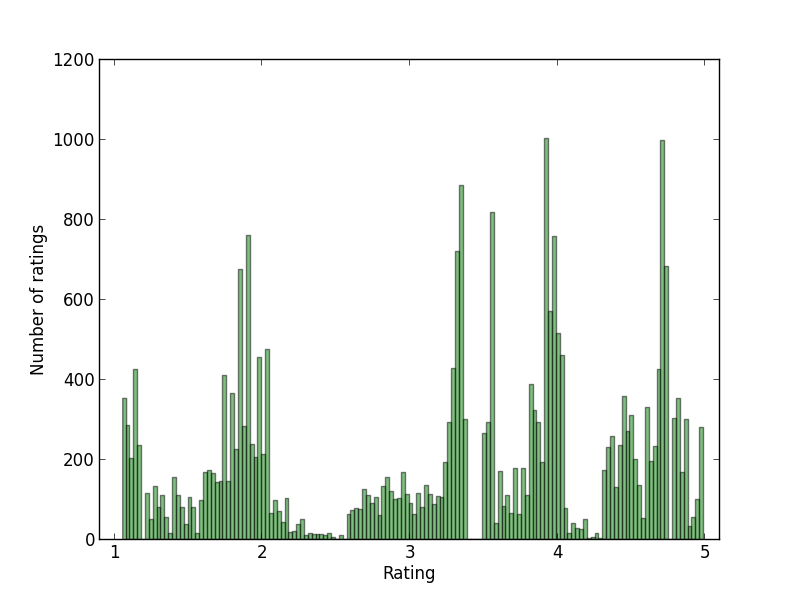
\includegraphics[scale=0.5]{image/dist-sigmoid-fixed-recentness-3-5}
  \caption{Distribution of ratings using number of days since earliest event,
  a logistic penalization function and global min/max feature-values}
  \label{fig:dist-recentness-sigmoid}
\end{figure}

As discussed in the previous section, using number of days since most recent
event has many weaknesses, most notably the returning user - who if absent for
a longer time finds all items previously viewed or bought heavily penalized.
Instead we can use the ordering of items with a logistic penalization function
as well. Continuing with a ratio of $3.5$ we obtain the following distribution:

\begin{figure}[H]
  \centering
  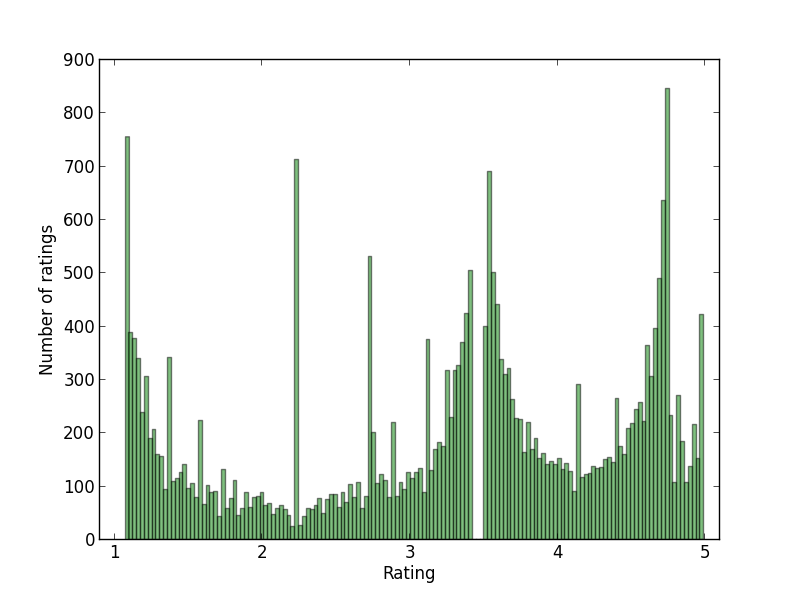
\includegraphics[scale=0.5]{image/dist-sigmoid-fixed-count-3-5}
  \caption{Distribution using ordering of events, a logistic penalization
  function and global min/max feature-values}
  \label{fig:dist-count-sigmoid}
\end{figure}

\subsection{Considering price}

In the same manner as with recentness we want to consider other features
apparent in our data and domain. As seen in Figure~\ref{} there is, not
surprisingly, a difference between users in average price on items they
frequent. Utilizing this variance we can create personalized ratings where we
try to give high ratings to items in the same price class as the user,
penalizing products that are too expensive or cheap.

The procedure is done in two steps: first we find the average price $a_u$ on
all items related to the user $u$. In the second step we make a second pass
over all items the user has shown interest in and calculate the distance to
$a_u$, yielding $x = p_i - a_u$ where $p_i$ is the price of item $i$. We then
find the penalization by:

\begin{equation}
  p(x,u) = \min{1, \frac{x}{M}}
\end{equation}

where $M$ is a constant controlling at which point the difference in price
should be fully penalized. In our experiments setting $M = 1500$ worked well,
hence making a price difference of $1500$ or more fully penalized yielding a
rating of 1.

Before applying the penalization function we make the assumption that an item
having the price difference $x = -d$ (cheaper) should be penalized less than an
item with the price difference $x = d$ (more expensive). Further we want to
make the value $x$ absolute, before calculating the penalization since $0 \leq
p(x,u) \leq 1$. In conclusion we apply $x = |\frac{x}{2}|$ $\text{if}$ $ x < 0$
making cheaper items half as sensitive to penalization, compared to more
expensive items.

\begin{figure}[H]
  \centering
  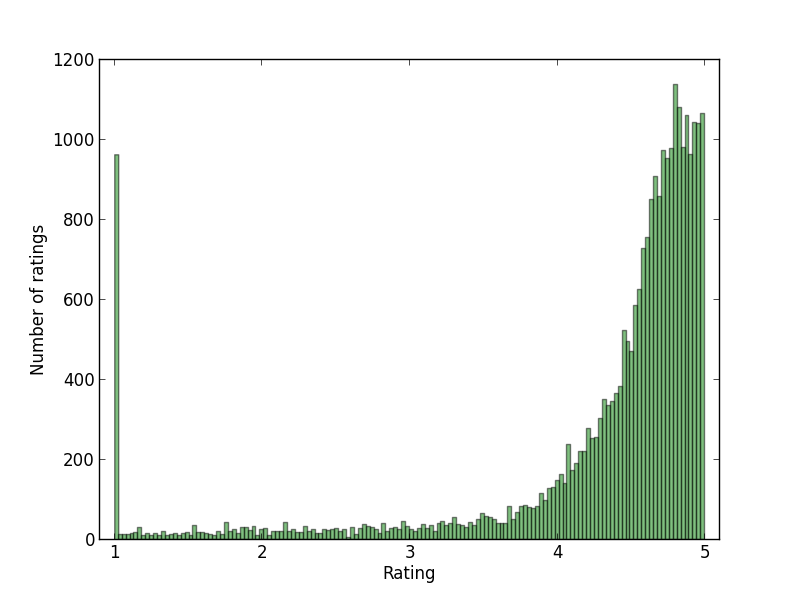
\includegraphics[scale=0.5]{image/dist-price}
  \caption{Distribution considering item price differences and each users conformity to
  its average price}
  \label{fig:dist-price}
\end{figure}

As seen the many items are penalized heavily for being to expensive, but this
is by design as we do not want to show too expensive items to the user
according to our assumptions. By setting $M$ higher, the number of items with
rating $1$ can be reduced. In addition most items gets a rating $5$ which tells
us that many users share the price preferences and by penalizing harder we can
reduce the number of items with rating 5. However, as we will see in subsequent
sections we are quite happy with the above distribution.

\subsection{Considering item popularity}

By looking at the global popularity of all item we can essentially tell if a
users activities classifies as conforming to the common standards or if the
users event patterns are more \textit{unique}. Our goal is to first classify to
which degree a user like globally popular items and then give penalizations to
items that are \textit{too popular} (the user is not adhering to peer-pressure)
or \textit{too obscure} (the user prefers popular items).

By first sorting all products by the number of related events we assign
a popularity score $0 \leq p \leq 1$, where $p=0$ is the product with the most
events and $p=1$ the event with the least number of events. Then we calculate
the average popularity score $a_e$ across all events, yielding $a_e = 0.76$.

In order to find a good penalization function we looked for the following
properties:

\begin{itemize}
  \item The top-value of $y$ should be at $x = 0.76$.
  \item When $x = 0$, that is for the most popular item, we should not penalize
  with $1.0$ nor $0.0$. A value of $y = 0.5$ was chosen.
  \item At $x = 1$ we want $y = 1$, giving maximum penalization to
  inpopular items.
\end{itemize}

And settled for having two linear functions, one when the popularity of item
$i$ was below the average popularity ($p_i < a_e$) and the second for when the
popularity was equal or higher.

\begin{equation}
  p(x, u) =
    \begin{cases}
      -\frac{c}{a_e}x + c                     & \text{if } x < a_e \\[1.5ex]
      \frac{1}{1-a_e}x - \frac{1}{1-a_e} + 1  & \text{if } x \geq 0
    \end{cases}
\end{equation}

where $c$ is the value chosen as penalization to the most popular item. As
mentioned this was in our experiments set to $0.5$. Using the SoBazaar $a_e$ we
obtained the following distribution and penalization function after
normalization:

\begin{figure}[H]
  \begin{subfigure}[b]{0.56\textwidth}
    \centering
    \resizebox{\linewidth}{!}{
      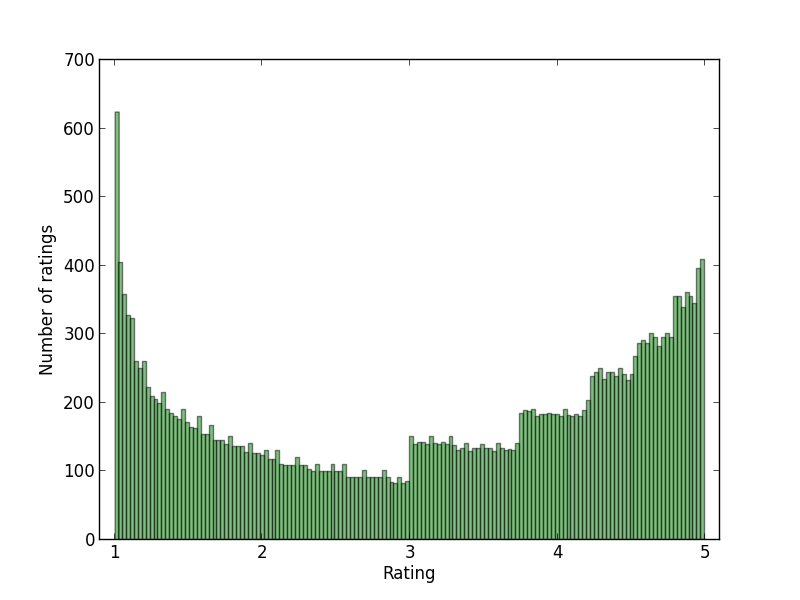
\includegraphics{image/dist-popularity}
    }
  \end{subfigure}
  \begin{subfigure}[b]{0.5\textwidth}
    \centering
    \resizebox{\linewidth}{!}{
      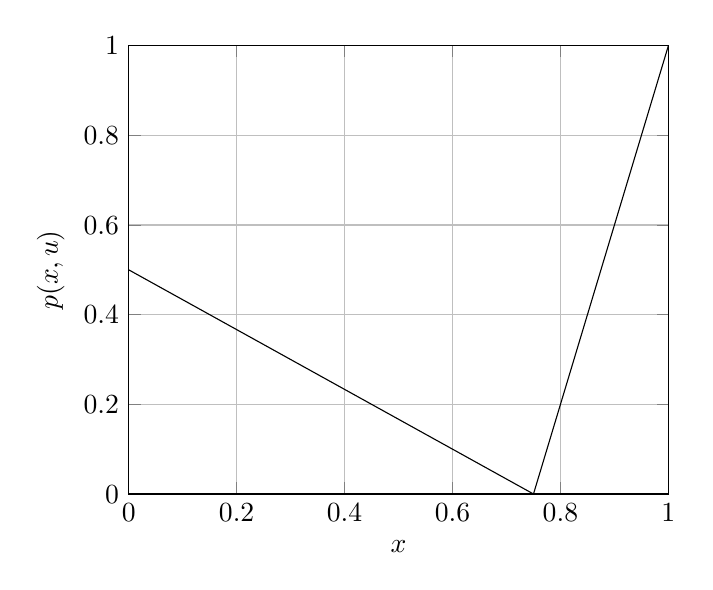
\begin{tikzpicture}
        \begin{axis}[
          ymin=0,ymax=1,
          xmin=0,xmax=1,
          grid=both,
          xlabel=$x$,
          ylabel={$p(x,u)$}
        ]
          \addplot[black] {-0.5/0.75*x + 0.5};
          \addplot[black] {1/(1-0.75)*x - 1/(1-0.75) + 1};
        \end{axis}
      \end{tikzpicture}
    }
  \end{subfigure}
  \caption{Distribution and penalization function, considering item popularity
  and the users conformity to popular items}
  \label{fig:dist-popularity}
\end{figure}

The peak at rating $1$ is a result of many items having close to zero events
connected to them. More interestingly we observe an evenly distributed spread
of ratings and, as with price, a peak at rating $5$ is expected as this is
given to the items close to the \textit{average} popularity.

\subsection{Linearly combining implicit ratings}

At this point we have found multiple ways of calculating the implicit ratings,
based on our implicit feedback. However, each method has its weaknesses,
strengths and captures different feature-sets in our data. Thus the
distributions reflect a large difference in ratings. Selecting a feature such
as number of days since the event in question captures our implicit knowledge
about seasons and items having a short life-span. However, as pointed out
earlier given many events on the same day there are no way of differentiating
them - unless we consider the ordering of items, saying the most recent item
shall be higher rated than older events. However, exclusively changing the
feature like this forces us to loose some of our implicit data about items
having a fixed lifespan. What we want to do is \textit{combine the two
features} in a procedure that often in recommender systems are coined
\textit{blending} or \textit{ensemble methods}. Combining them enables us to
create more robust ratings where weaknesses such as outliers or inconsistencies
in one method can be averaged out by the strengths of others. If two features
independently finds the same properties and ratings for some items and users,
then the result and our belief is strengthened.

When linearly combining $M$ models $m_1 \dots m_M$, we choose $M$ factors $f_i$
all adding up to 1.0, representing the weight of model $m_{i}$ in the final
\textit{blend}. Each model then have $k$ ratings on the triplet form
\textit{(user, product, rating)} and noted noted as $r_{ij}$ - the rating of
item $j$ in model $i$.

Then when calculating the final rating for item $j$ we sum over all
models:

\begin{equation}
  r_j = \sum _{i=1}^{M} f_{i} * r_{ij}
\end{equation}

Given two models, we can observe the result of performing a blend between with
factors $f_1 = 0.7$ and $f_2 = 0.3$ and the two ratings $r_{11} = 5$ and
$m_{21} = 3$ for a given item, we can calculate the final rating as $(0.7
\times 5) + (0.3 \times 3) = 4.4$. The obvious weakness in this approach is the
need for manually setting weights for $M$ different factors. Optimally we would
like to run one blend, look at the result, compare it to previous results and
make adjustments to the weights based these. This is what is done in simple
blending schemes using Linear Regression or KNN, but many state-of-the-art
schemes exists as well such as Binned Linear Regression, Bagged Gradient
Boosted Decision Tree (BGBDT), Neural Networks and Kernel Ridge Regression
Blending \cite{jahrer2010combining} \cite{toscher2009bigchaos} which are based
on the same principles.

However, as discussed in Section~\ref{}, when creating ratings from implicit
feedback we lack a ground truth --- that is we make several assumptions on which
implicit features contribute towards higher preference and thus higher ratings,
but with no real means of confirming the assumptions. A user buying an item as
a gift for a friend may not actually like the item and would not give a high
rating - and this, with a traditional collaborative filtering approach based on
explicit feedback would be accounted for, looking at the user pattern of the
user and labeling the purchase as an outlier. Without this ground truth however
we can not without injecting negative feedback, based on assumptions, make
classifications of outliers nor evaluate our implicit ratings in a reliable and
quantiative fashion. Without a good evaluation metric and grund truth there
does not exists a simple way of comparing different blends with eachothers
neither, hence making it difficult to find custom weights for each method.

Instead, we return to our introductionary text where we notice some factors
important to evaluating ratings: it needs to be evenly distributed, it should
have an average confirming our hypthesis and the features selected should
capture properties found in the domain both intutivly and quantitativly.  Then
for $M$ different models we assume they all contribute an equal amount to the
final results thus having the weights $f_i = 1/M$.

\subsubsection{Combining recentness features}

We can combine our methods looking at recentness using a linear penalization
function (Figure~\ref{fig:dist-recentness-linear-global}
and~\ref{fig:dist-count-linear}) and with the ratings generated with a logistic
penalization function (Figure~\ref{fig:dist-recentness-sigmoid}
and~\ref{fig:dist-count-sigmoid}) looking at both days and ordering of events.
This yields the following distribution of ratings with the average $3.30$ and
median at $3.63$, where the distributions overlayed with the kernel density
function, showing the trend of histogram:

\begin{figure}[H]
  \centering
  \label{dist-blend}
  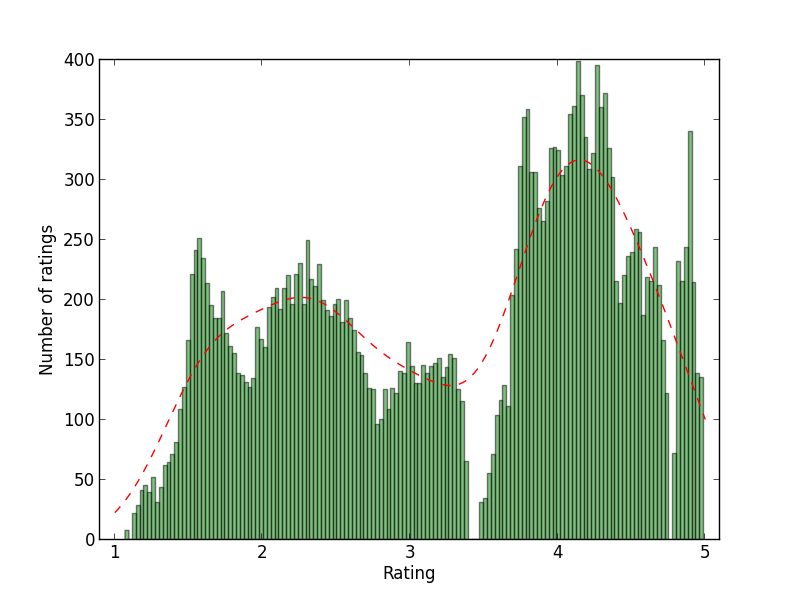
\includegraphics[scale=0.5]{image/dist-blend}
  \caption{Distribution using blend of ordering and number of days since event,
  with logistic and linear penalization functions, overlayed with density
  function}
\end{figure}

Especially noticable in this distribution is that we've achieved a even
distribution without too many fluxuations. In addition there is a rounded peak
aroung the rating 4, which by looking at other public datasets such as in the
Netflix Prize~\cite{Netflix} or Million Song Dataset~\cite{Bertin-Mahieux-2011}
is a common peak found in explicit environments. Indeed, there is a small gap
where the scores between our two events \textit{click} and \textit{want} are
bordering, a result of our sigmoid functions having a ratio of $3.5$ which
yields a gradual slope - hence when we have x-values close to $M_u$ and $0$ we
approximate $1$ and $0$ respectivly, but we do not reach it exactly. This can
be seen on Figure~\ref{fig:sigmoid-penalizations}

\subsubsection{Combining recentness, popularity and price}

Instead of only looking at recentness, we can combine it with our other
features found in the previous section - namely price and popularity, as well.
As we saw by Figure~\ref{dist-price} and Figure~\ref{dist-popularity}, the
distribution of ratings considering both prices and popularities respectivly
have peaks at edge values $1$ and $5$. When combined an item with high rating
in regards to price, but low rating considering popularity will be lowered to a
rating around $3$ - and if features are chosen coherent to what we expect the
data to represent, we expect to see a final blend where most ratings are
allocated a value around $3-4$ with few or none gaps.

\begin{figure}[H]
  \centering
  \label{dist-blend-price}
  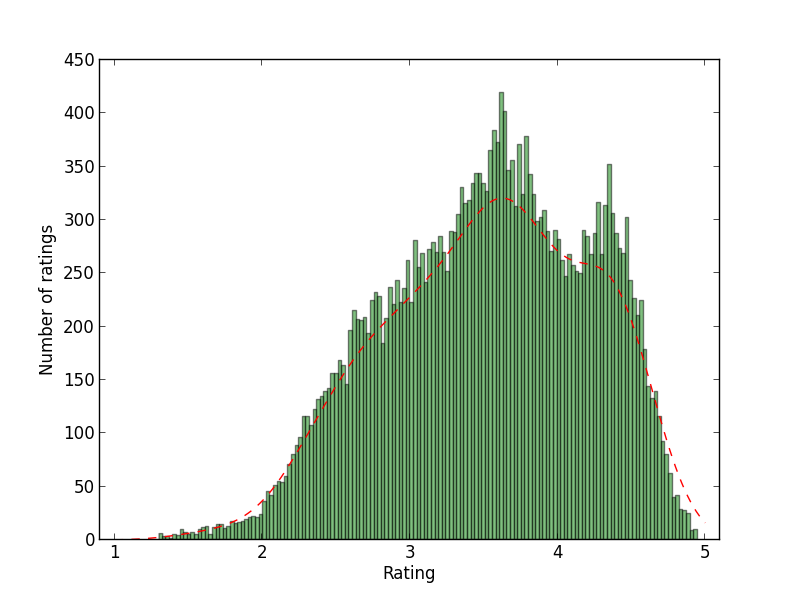
\includegraphics[scale=0.5]{image/dist-blend-price-popularity-recentness}
  \caption{Distribution using blend of price, popularity and recentness with
  linear penalization, overlayed with density function}
\end{figure}

By here combinging ratings generated by recentness (both ordering and age of
events), popularity and price we see our so far "best" distribution in terms of
non quantifiable metrics. The distribution has an average rating of $3.5305$
and median $3.5780$, indicating an even spread. In the above example we have
used logistic penalization functions with constant $3.5$ as depicted in
Figure~\ref{dist-recentness-sigmoid} and~\ref{dist-count-sigmoid}. Using a
linear penalization function instead yields the average value $3.5293$ and
median $3.5883$, hence no large difference. The logistic approach was however
considered superior and used in future experiments as it captures the linearity
of the data, whilst in the same time accounting for seasons and the life span
of items seen in the fashion domain.

% Perhaps tell something about experiemnts that led us to choose sigmoid >
% linear?
% Any more comments on this one?
